\documentclass{beamer}
\usepackage{graphicx}
\usepackage{amsmath}

\title{Detailed Explanations of Fiscal Policy Concepts}
\author{Charles Ancel}
\date{July 24, 2024}

\begin{document}

\frame{\titlepage}

\section{Introduction}
\begin{frame}
    \frametitle{Introduction}
    My name is Charles Ancel, my UIN is 654604114, and this is my ID. I'm currently enrolled in ECON 425 during the Summer Session. This assignment is part of the requirement from the University regarding the College of LAS's identity verification policy for LAS Online-certified classes. For the answers in this assignment, I did not use any form of Artificial Intelligence (AI) help, such as Chat-GPT or similar, and thus my answers will accurately and fairly reflect my own learning from this course.
\end{frame}

\section{Ricardian Equivalence}

\begin{frame}
    \frametitle{Ricardian Equivalence}
    \begin{itemize}
        \item \textbf{Statement:} ``I don't believe in the Ricardian equivalence, why should anybody care about learning such a thing? I think that it is devoid of any substance and thus I see it as a complete waste of time.''
    \end{itemize}
\end{frame}

\begin{frame}
    \frametitle{Understanding Ricardian Equivalence}
    \begin{itemize}
        \item \textbf{Theory:} Suggests that financing government spending with debt rather than taxes does not affect overall demand.
        \item \textbf{Rational Consumers:} Anticipate future taxes to pay off debt, thus saving more and offsetting increased demand.
    \end{itemize}
\end{frame}

\begin{frame}
    \frametitle{Importance of Ricardian Equivalence}
    \begin{itemize}
        \item \textbf{Policy Impact Analysis:} Helps evaluate long-term effects of government borrowing.
        \item \textbf{Consumer Behavior:} Provides insights into responses to fiscal policy changes.
        \item \textbf{Fiscal Responsibility:} Highlights future tax burdens in debt-financed policies.
    \end{itemize}
\end{frame}

\begin{frame}
    \frametitle{Diagram of Ricardian Equivalence}
    \begin{figure}[h!]
        \centering
        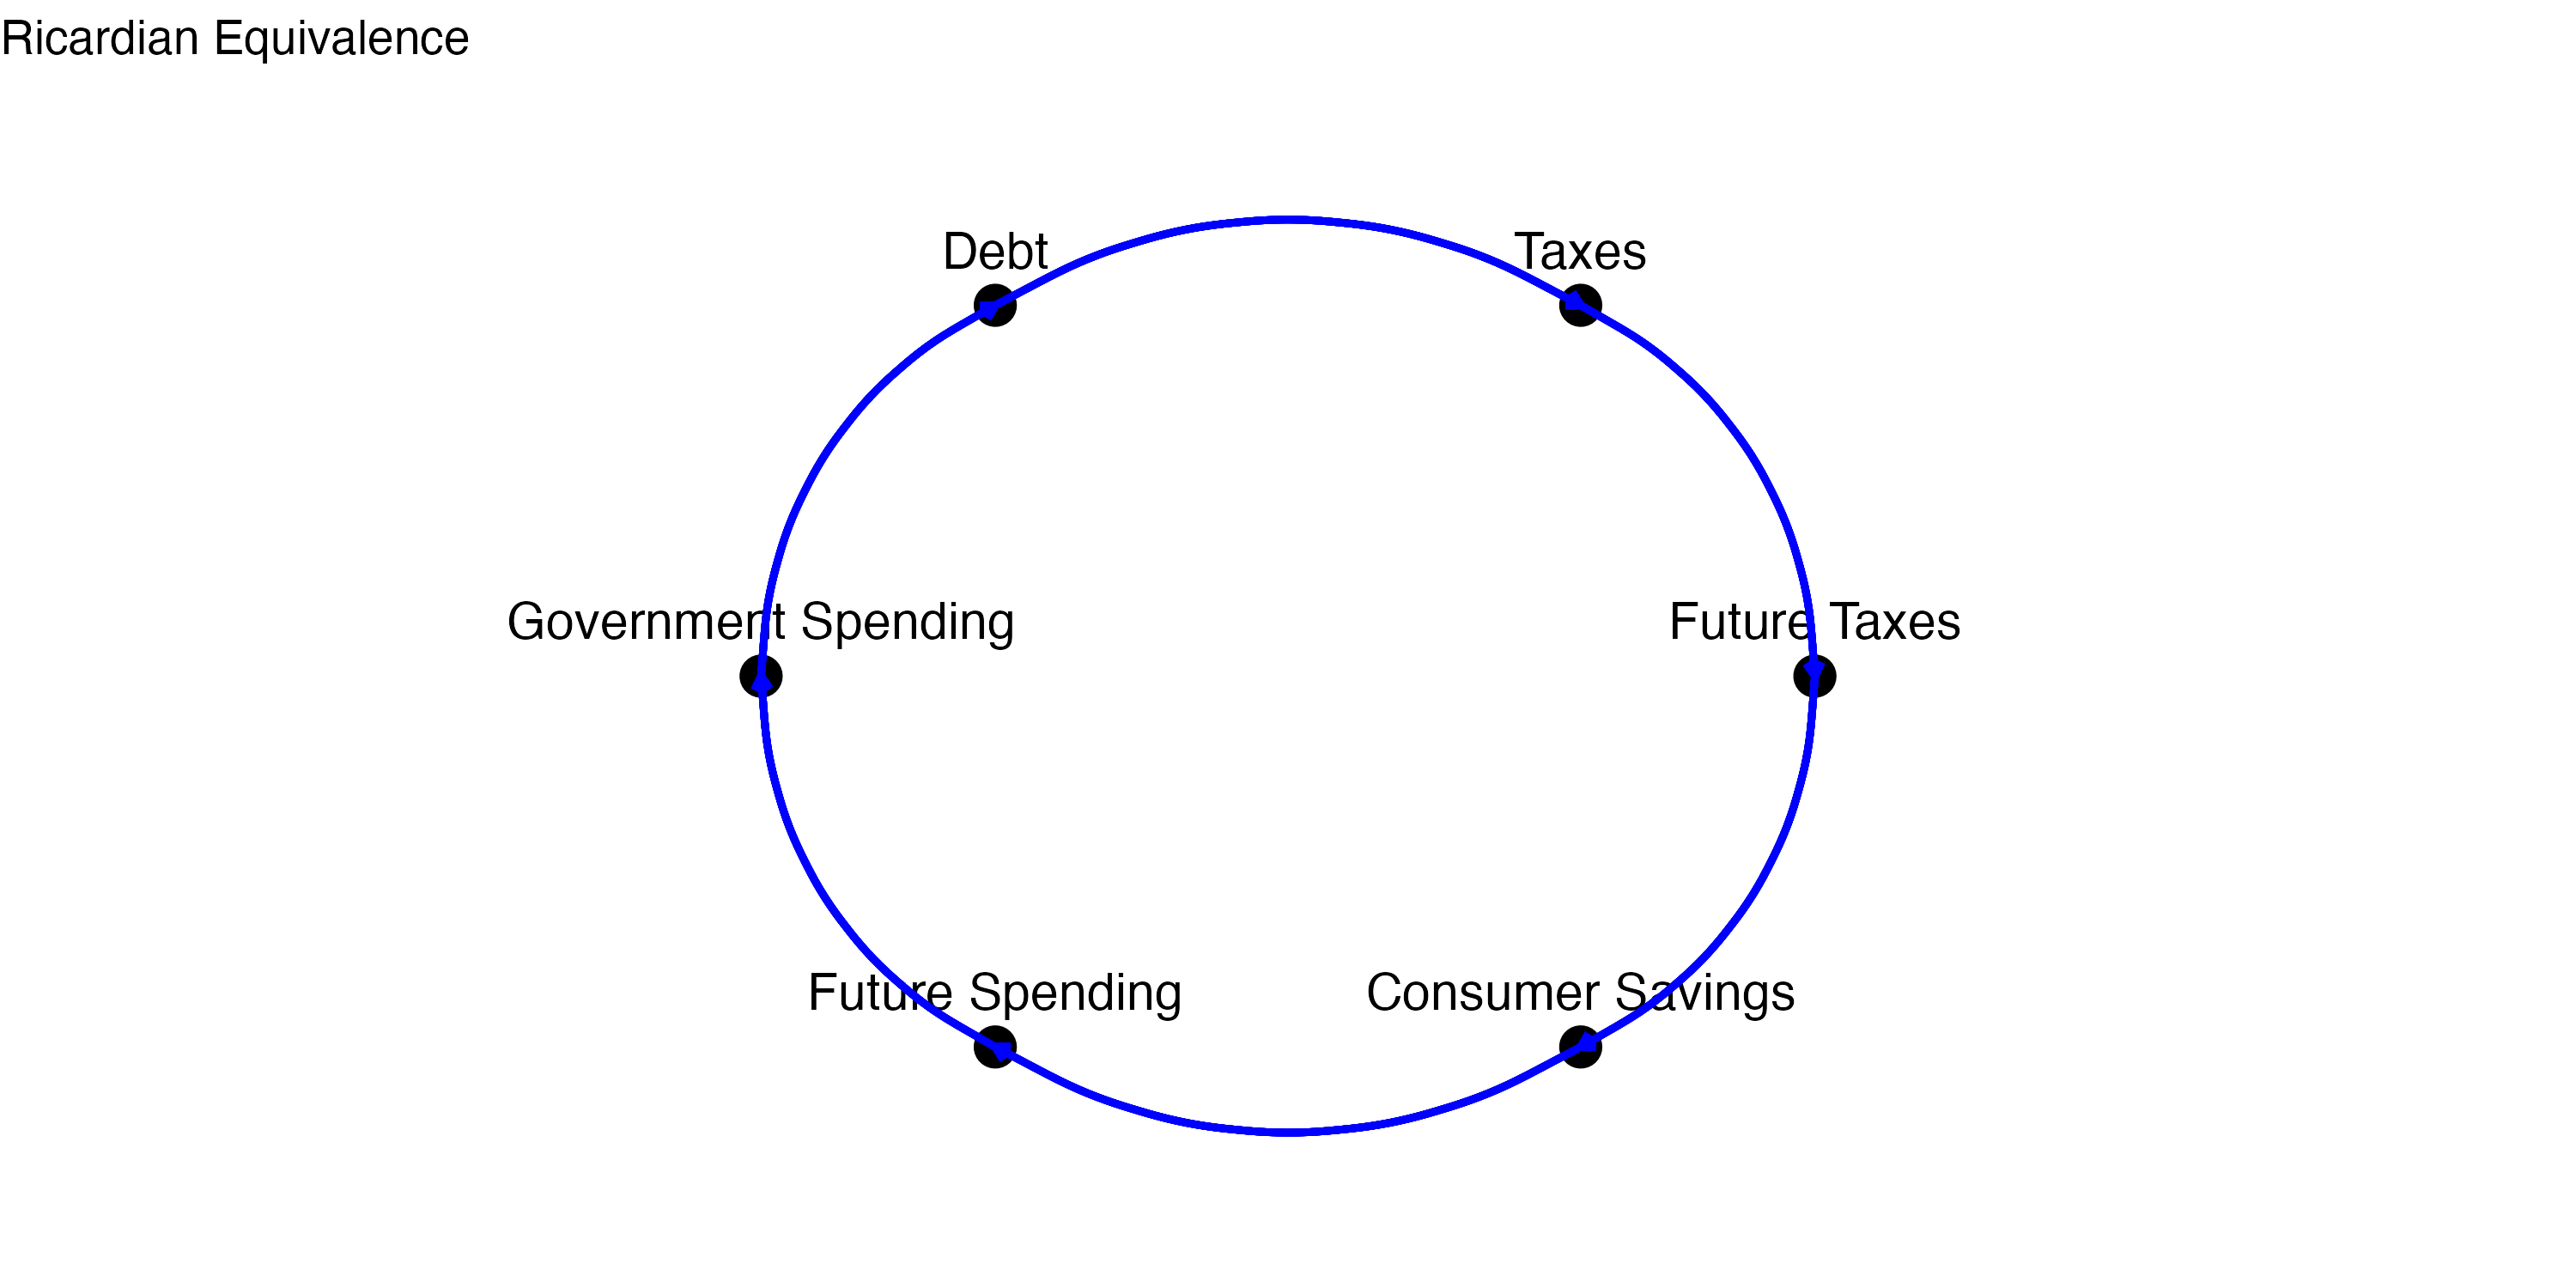
\includegraphics[width=1.2\textwidth]{/Users/cancel/Personal/Coursework/Econ425/VA3/R/Ricardian_Equivalence.png}
    \end{figure}
\end{frame}

\begin{frame}
    \frametitle{Key Takeaways: Ricardian Equivalence}
    \textbf{Key Takeaways:}
    \begin{itemize}
        \item Helps in understanding consumer behavior in response to fiscal policy.
        \item Highlights the importance of future tax burdens in fiscal policy decisions.
        \item While theoretical, provides a basis for policy impact analysis.
    \end{itemize}
\end{frame}

\section{Government Deficit and Constraints}

\begin{frame}
    \frametitle{Government Deficit and Constraints}
    \begin{itemize}
        \item \textbf{Statement:} ``I've read this book written by a Twitter celebrity that says the government can increase its deficit forever without any actual constraint. Why is not the government doing that already?''
    \end{itemize}
\end{frame}

\begin{frame}
    \frametitle{Constraints on Government Deficits}
    \begin{itemize}
        \item \textbf{Debt Sustainability:} Continuous deficits increase national debt, potentially becoming unsustainable.
        \item \textbf{Inflation:} Large and persistent deficits can lead to inflation if demand exceeds productive capacity.
        \item \textbf{Market Confidence:} Financial markets may lose confidence, increasing borrowing costs and economic instability.
    \end{itemize}
\end{frame}

\begin{frame}
    \frametitle{Government Debt and Interest Rate}
    \begin{figure}[h!]
        \centering
        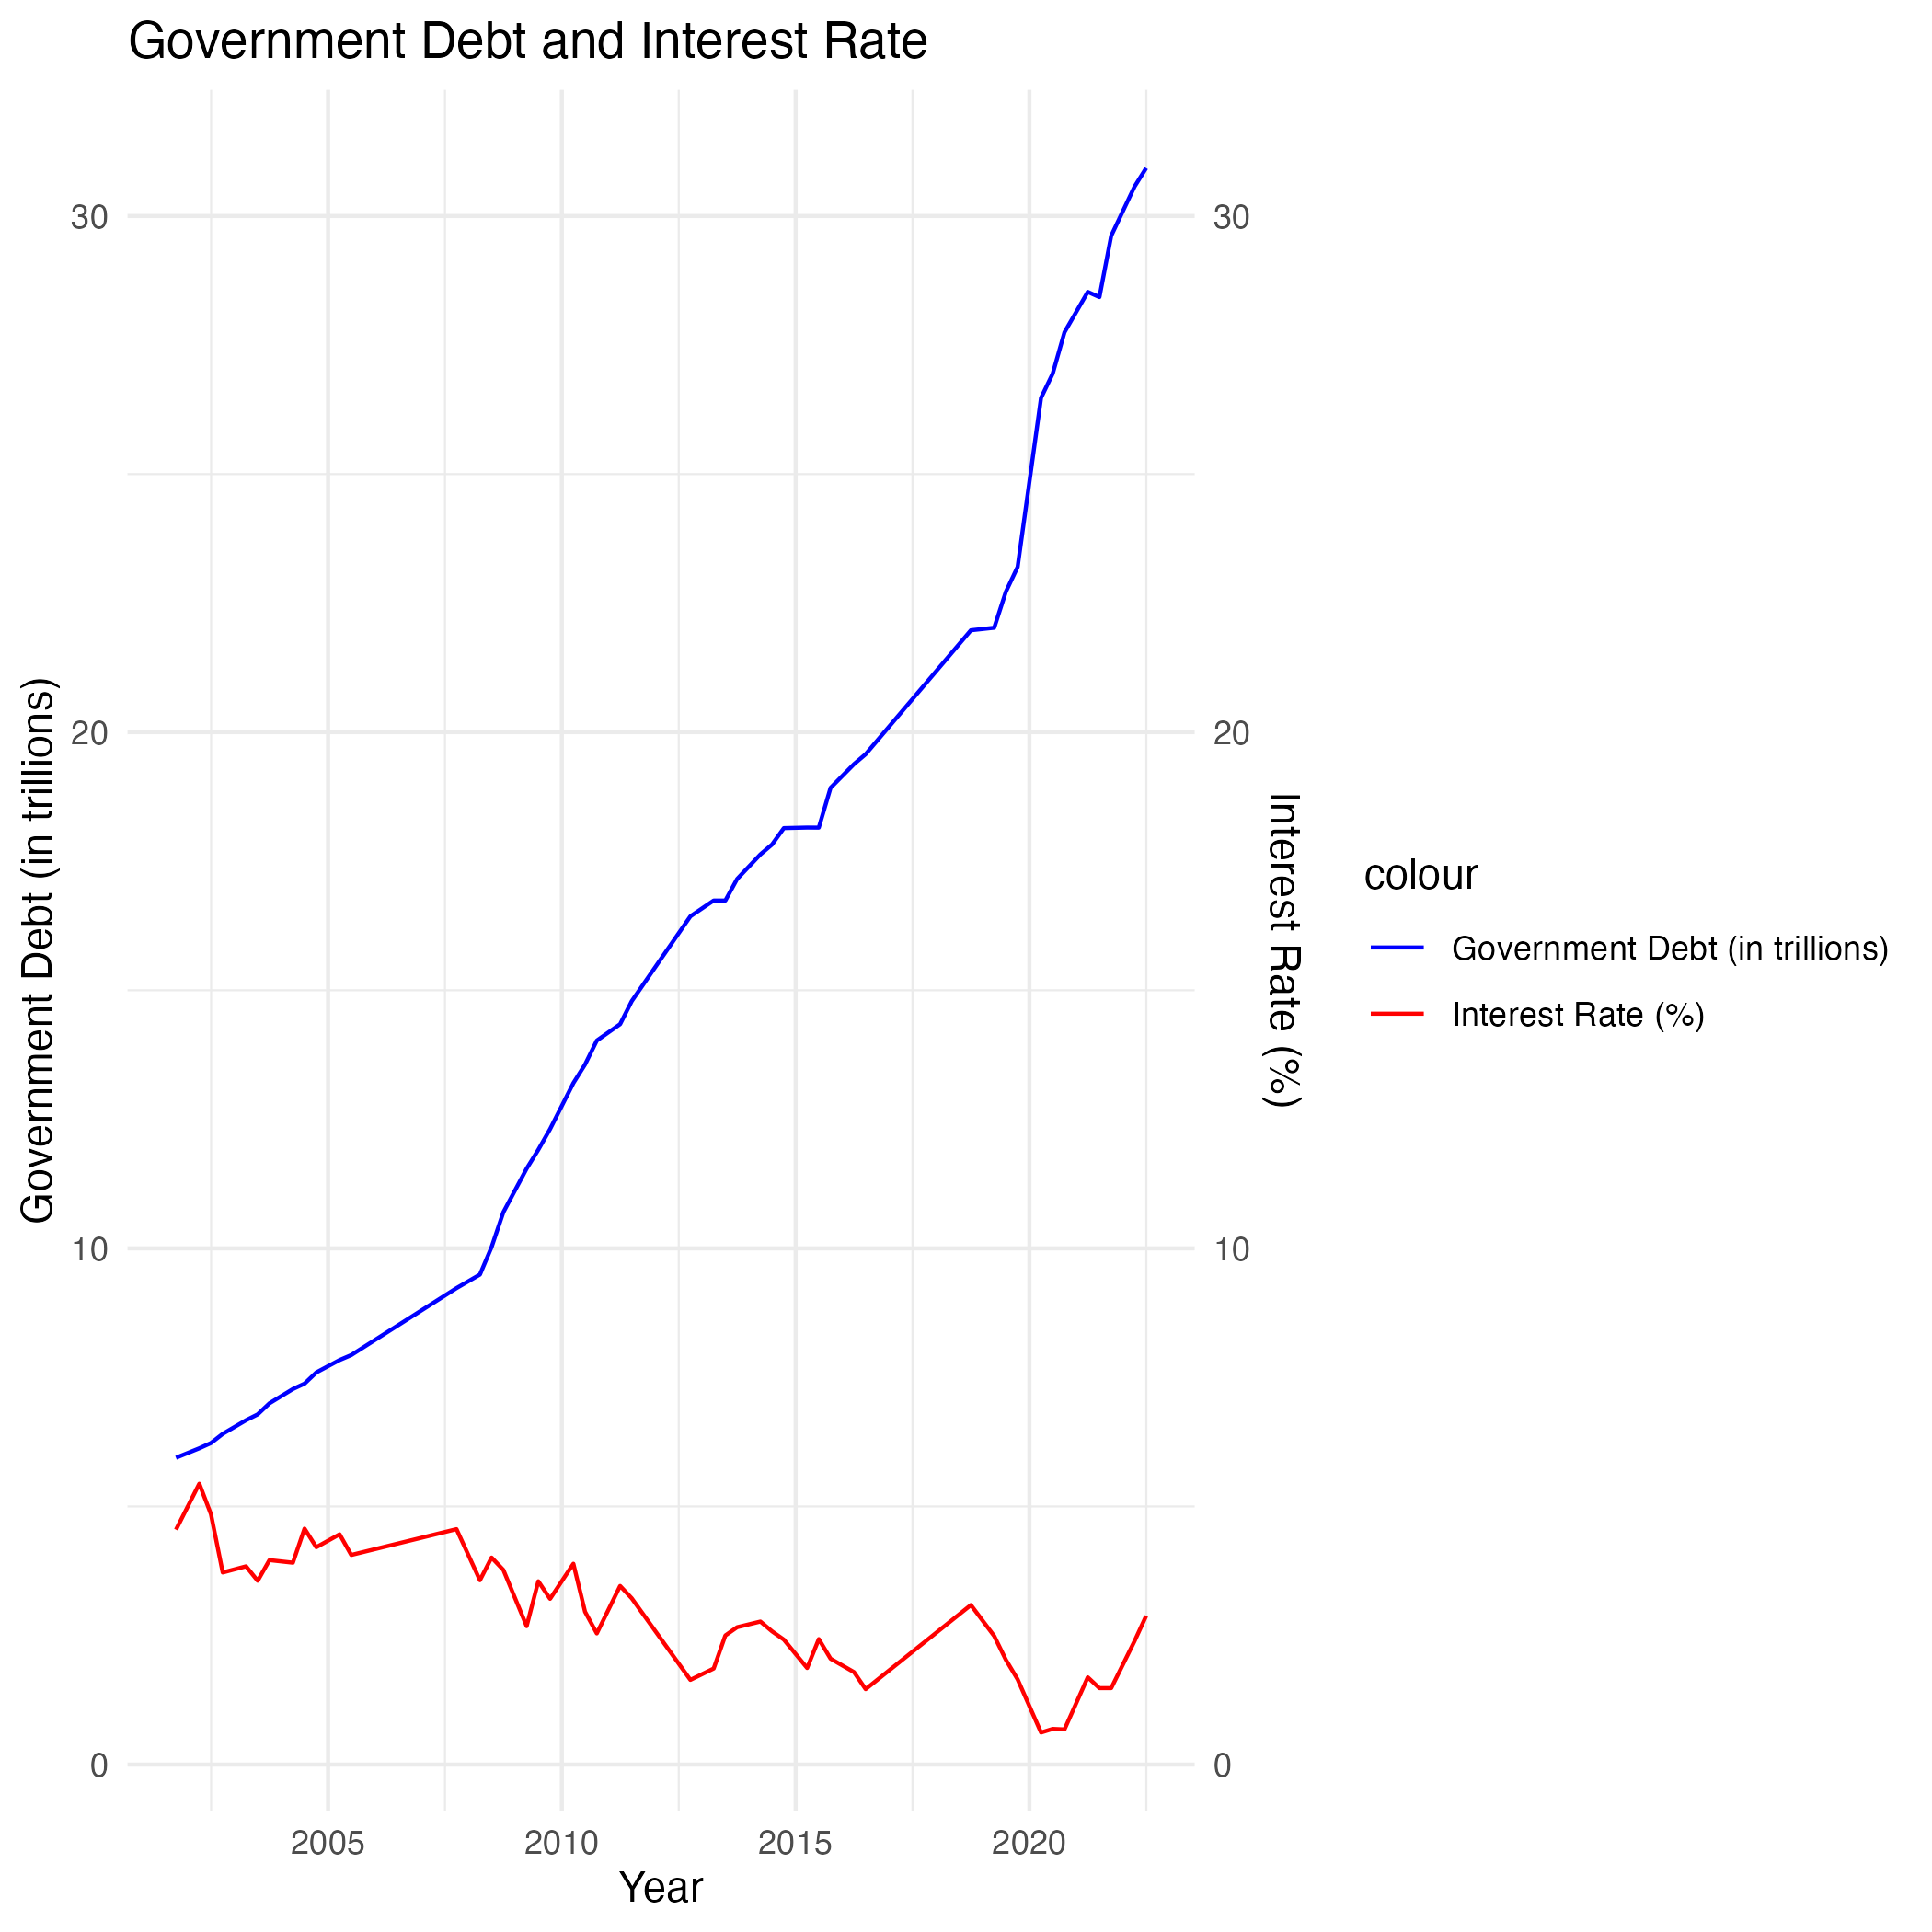
\includegraphics[width=0.8\textwidth]{/Users/cancel/Personal/Coursework/Econ425/VA3/R/Debt_Constraints.png}
    \end{figure}
\end{frame}

\begin{frame}
    \frametitle{Key Takeaways: Government Deficit and Constraints}
    \textbf{Key Takeaways:}
    \begin{itemize}
        \item Continuous deficits can lead to unsustainable debt levels.
        \item High deficits can cause inflation and higher interest rates.
        \item Market confidence is crucial for maintaining stable borrowing costs.
    \end{itemize}
\end{frame}

\section{General Equilibrium Models}

\begin{frame}
    \frametitle{General Equilibrium Models}
    \begin{itemize}
        \item \textbf{Statement:} ``General equilibrium models are not helpful to understand fiscal policy because they are too simplistic, the real world is at odds with such models. Furthermore, with the Big Data availability that we have now, models are no longer required.''
    \end{itemize}
\end{frame}

\begin{frame}
    \frametitle{Utility of General Equilibrium Models}
    \begin{itemize}
        \item \textbf{Analytical Framework:} Structured way to analyze interactions and responses to policy changes.
        \item \textbf{Policy Simulation:} Helps simulate potential impacts before implementation.
        \item \textbf{Complement to Big Data:} Enhances model accuracy with detailed and real-time data inputs.
    \end{itemize}
\end{frame}

\begin{frame}
    \frametitle{General Equilibrium Model}
    \begin{figure}[h!]
        \centering
        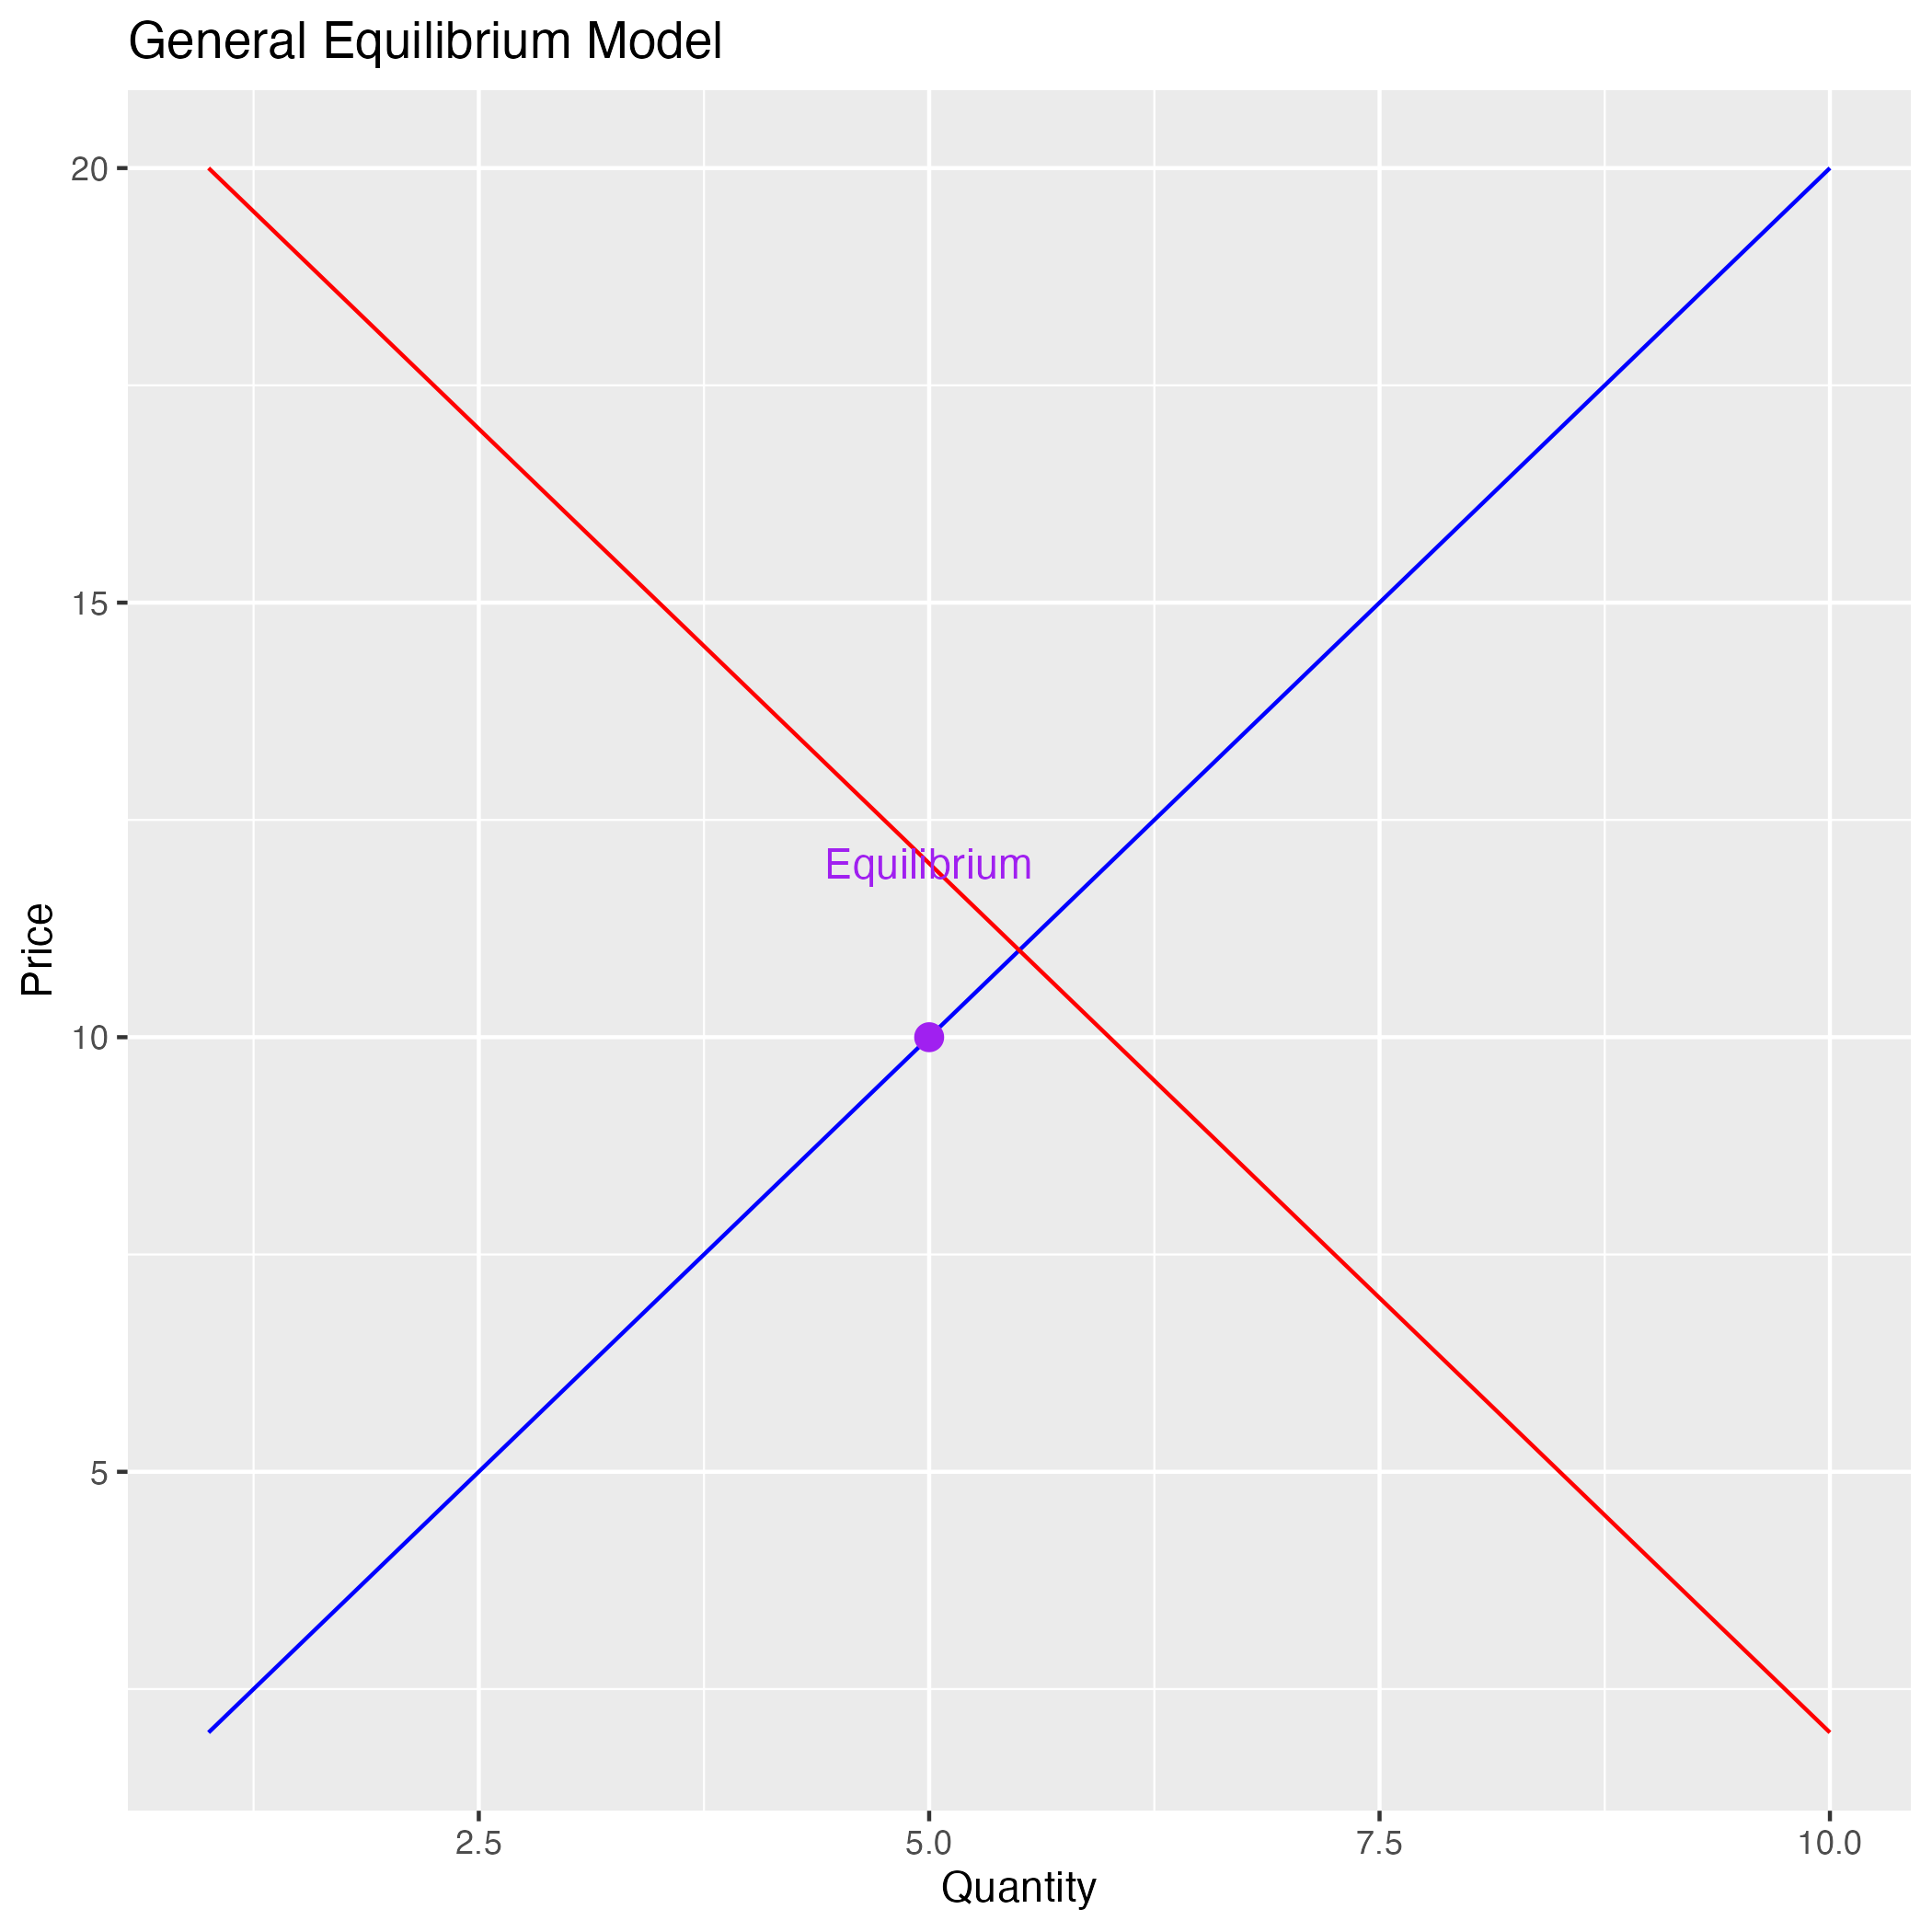
\includegraphics[width=0.8\textwidth]{/Users/cancel/Personal/Coursework/Econ425/VA3/R/General_Equilibrium.png}
    \end{figure}
\end{frame}

\begin{frame}
    \frametitle{Key Takeaways: General Equilibrium Models}
    \textbf{Key Takeaways:}
    \begin{itemize}
        \item Models provide a structured way to analyze economic interactions.
        \item They help in policy simulations and understanding potential impacts.
        \item Big Data complements but does not replace the need for theoretical models.
    \end{itemize}
\end{frame}

\section{Government Spending Multiplier}

\begin{frame}
    \frametitle{Government Spending Multiplier}
    \begin{itemize}
        \item \textbf{Statement:} ``I don't know why you say that the government spending multiplier is around 0.7 to 1.2. I read a piece of news that reported fiscal multipliers close to 2, and these were based on modern empirical research. Thus, we should fight for fiscal policies that push for the greatest government spending ever. Don't you think?''
    \end{itemize}
\end{frame}

\begin{frame}
    \frametitle{Understanding the Spending Multiplier}
    \begin{itemize}
        \item \textbf{Measurement:} Change in economic output from increased government spending.
        \item \textbf{Context-Dependent:} Value varies based on economic conditions and methodological approaches.
        \item \textbf{Policy Considerations:} Advocating maximum spending without considering nuances can lead to inefficiencies.
    \end{itemize}
\end{frame}

\begin{frame}
    \frametitle{Government Spending Multipliers}
    \begin{figure}[h!]
        \centering
        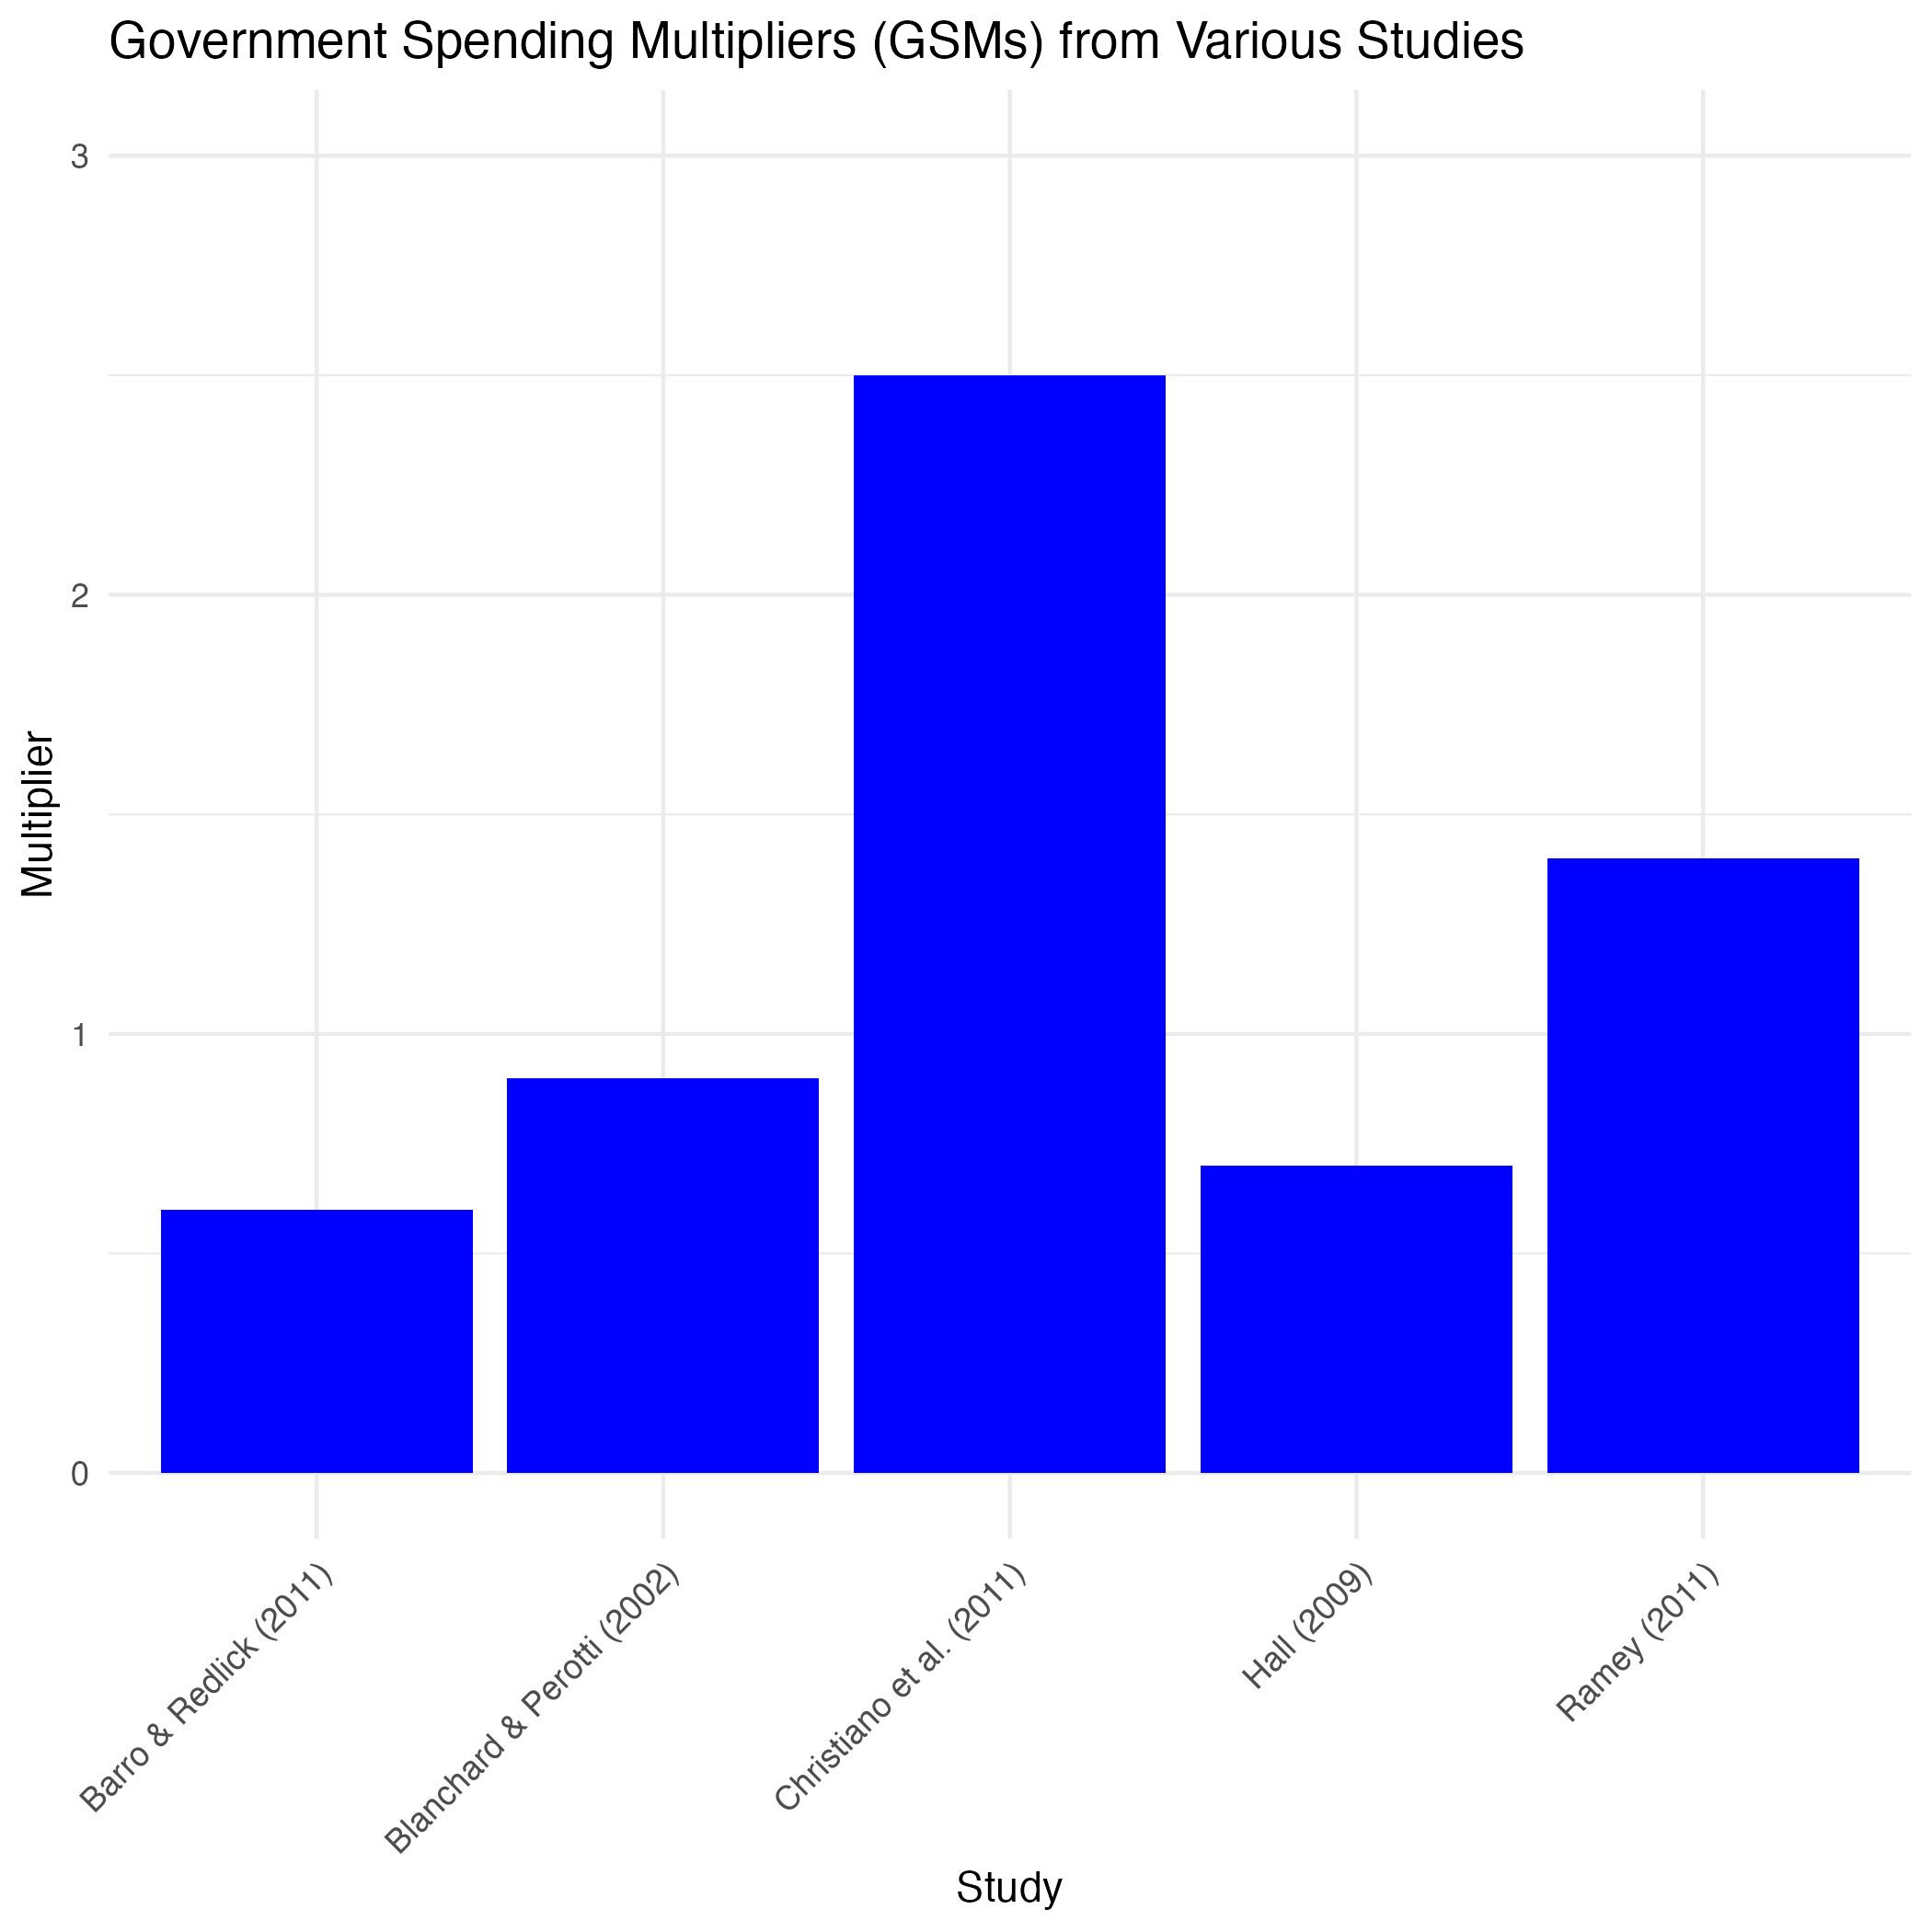
\includegraphics[width=0.8\textwidth]{/Users/cancel/Personal/Coursework/Econ425/VA3/R/Spending_Multipliers.png}
    \end{figure}
\end{frame}

\begin{frame}
    \frametitle{Key Takeaways: Government Spending Multiplier}
    \textbf{Key Takeaways:}
    \begin{itemize}
        \item Multiplier values depend on the economic context.
        \item Higher multipliers are more likely in a recession.
        \item Accurate estimation requires considering various economic conditions.
    \end{itemize}
\end{frame}

\section{Fiscal Multipliers and Income Tax Cuts}

\begin{frame}
    \frametitle{Fiscal Multipliers and Income Tax Cuts}
    \begin{itemize}
        \item \textbf{Statement:} ``If you insist that the government spending multiplier is around 1, we still have other fiscal multipliers we can use. Surely we can implement income tax cuts that cause effects that are as strong or even stronger than what we would get with government spending.''
    \end{itemize}
\end{frame}

\begin{frame}
    \frametitle{Effects of Income Tax Cuts}
    \begin{itemize}
        \item \textbf{Different Mechanisms:} Tax cuts increase disposable income, potentially boosting consumption and investment.
        \item \textbf{Distributional Effects:} Effectiveness varies across income groups.
        \item \textbf{Comparative Effectiveness:} Often lower multiplier than direct government spending, especially in economic slack.
    \end{itemize}
\end{frame}

\begin{frame}
    \frametitle{Fiscal Multipliers: Spending vs. Tax Cuts}
    \begin{figure}[h!]
        \centering
        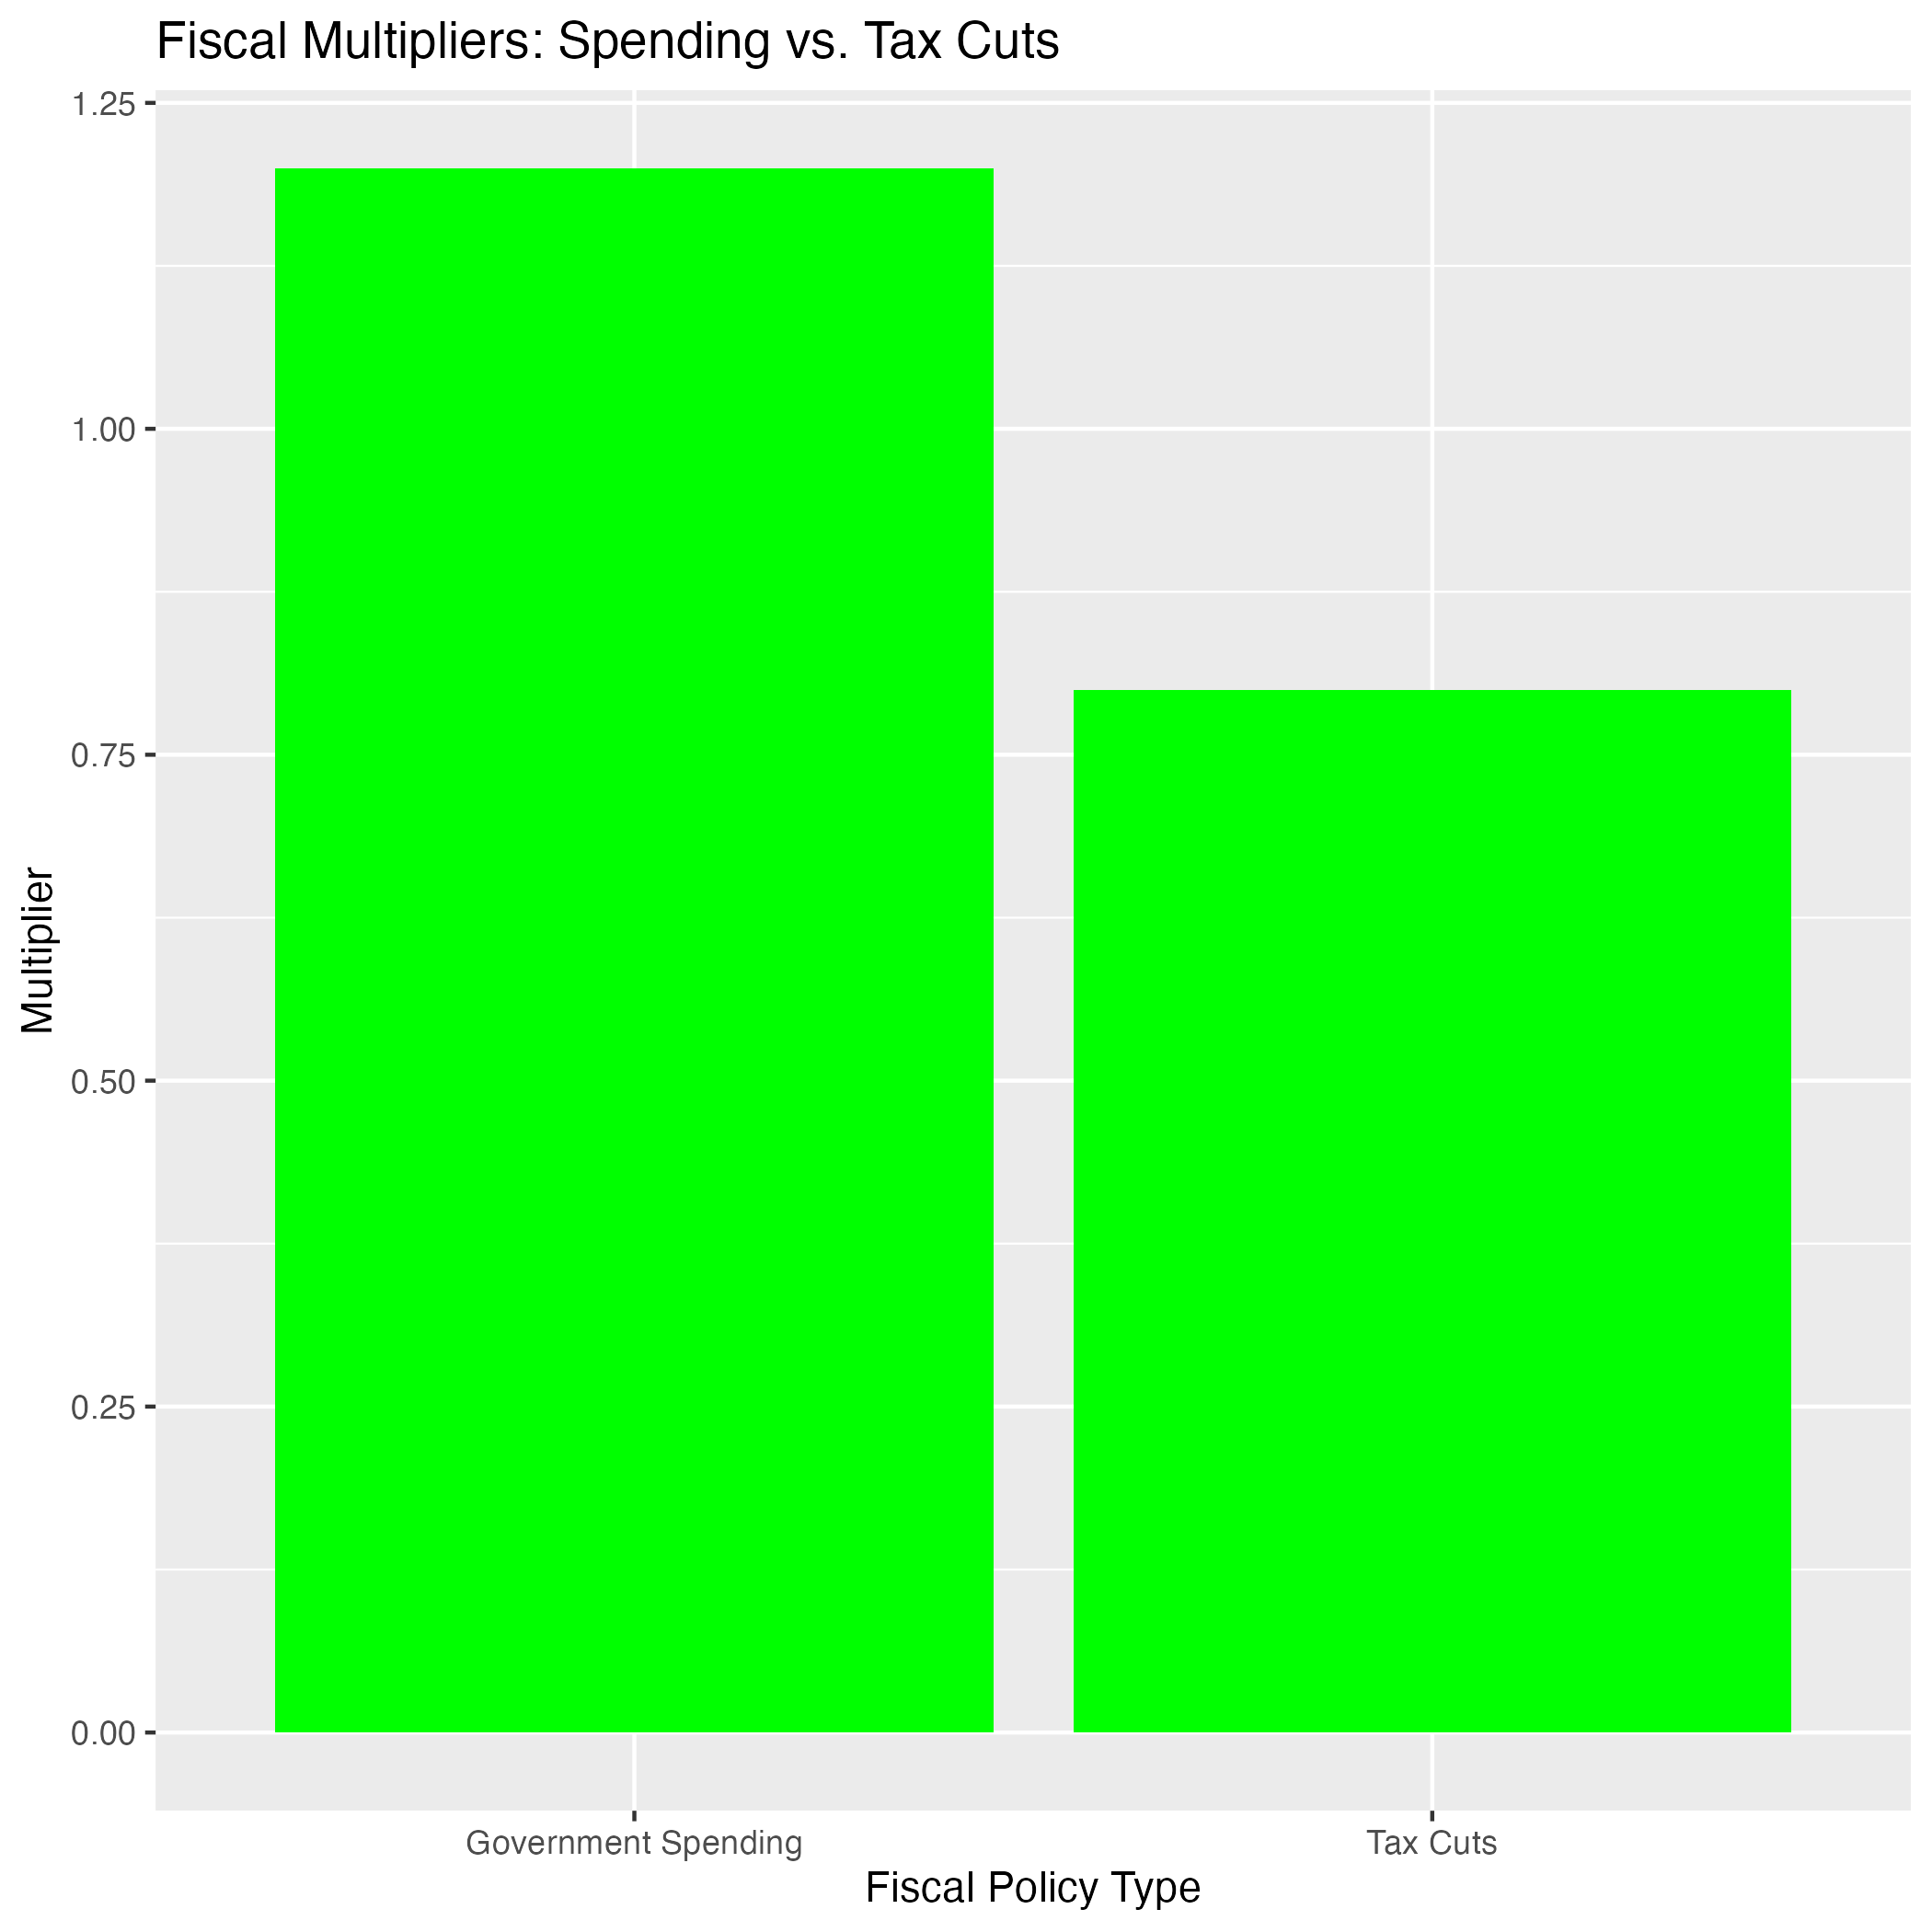
\includegraphics[width=0.8\textwidth]{/Users/cancel/Personal/Coursework/Econ425/VA3/R/Tax_Cuts_Multipliers.png}
    \end{figure}
\end{frame}

\begin{frame}
    \frametitle{Key Takeaways: Fiscal Multipliers and Tax Cuts}
    \textbf{Key Takeaways:}
    \begin{itemize}
        \item Tax cuts have different effects based on income distribution.
        \item Lower-income households are more likely to spend additional income.
        \item Government spending often has a higher immediate impact on GDP.
    \end{itemize}
\end{frame}

\section{VAT Cuts}

\begin{frame}
    \frametitle{VAT Cuts}
    \begin{itemize}
        \item \textbf{Statement:} ``Even if not, I heard from a friend, who is a serious economist, that we can always cut the VAT here in the US.''
    \end{itemize}
\end{frame}

\begin{frame}
    \frametitle{Considerations for VAT Cuts}
    \begin{itemize}
        \item \textbf{Limited Applicability:} The US does not have a federal VAT, though sales taxes at state and local levels function similarly.
        \item \textbf{Regressive Nature:} Sales tax cuts benefit higher-income households more.
        \item \textbf{Revenue Implications:} Reducing sales taxes decreases government revenue, impacting public services and investments.
    \end{itemize}
\end{frame}

\begin{frame}
    \frametitle{Impact of VAT Cuts}
    \begin{figure}[h!]
        \centering
        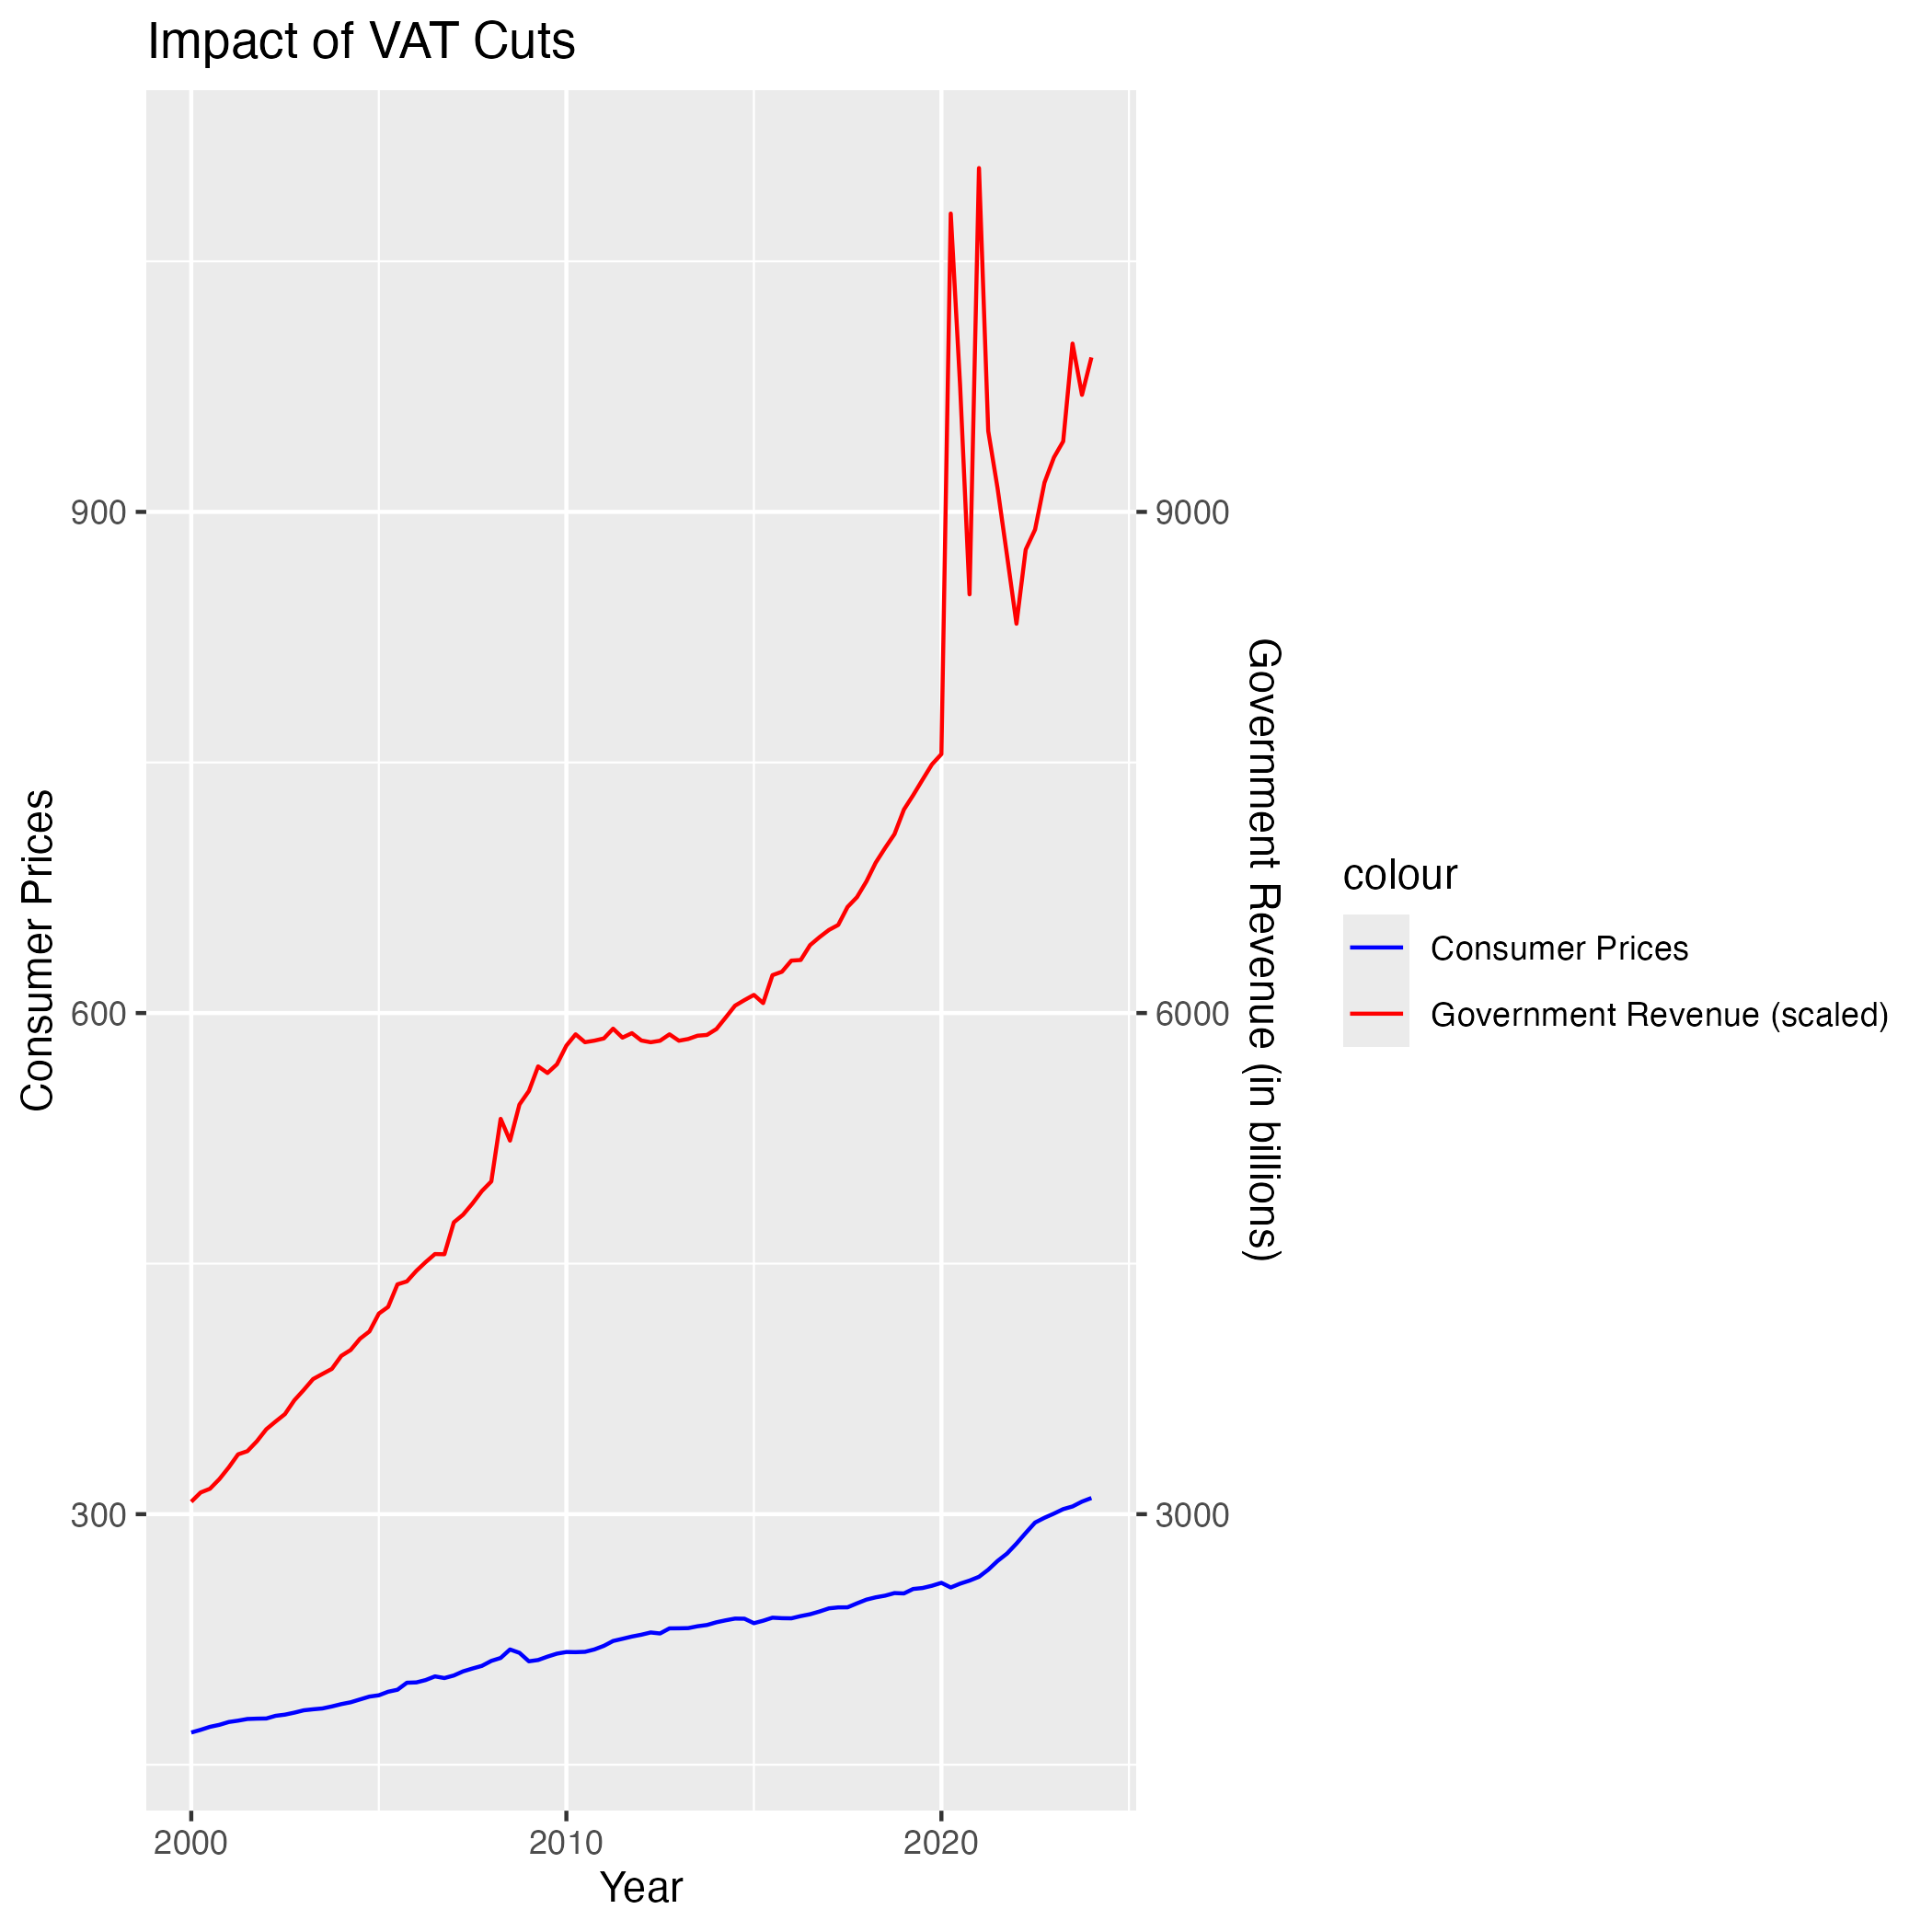
\includegraphics[width=0.8\textwidth]{/Users/cancel/Personal/Coursework/Econ425/VA3/R/VAT_Cuts_Impact.png}
    \end{figure}
\end{frame}

\begin{frame}
    \frametitle{Key Takeaways: VAT Cuts}
    \textbf{Key Takeaways:}
    \begin{itemize}
        \item VAT cuts can boost consumption but reduce government revenue.
        \item The impact on different income groups should be considered.
        \item Structural considerations are important for long-term fiscal health.
    \end{itemize}
\end{frame}

\section{Support for Fiscal Policy}

\begin{frame}
    \frametitle{Support for Fiscal Policy}
    \begin{itemize}
        \item \textbf{Statement:} ``Ok, ok. But then, you are probably against fiscal policy as a whole. How can you convince me that you are not just being political?''
    \end{itemize}
\end{frame}

\begin{frame}
    \frametitle{Defending Fiscal Policy}
    \begin{itemize}
        \item \textbf{Economic Stabilization:} Can counteract downturns by boosting demand.
        \item \textbf{Public Investment:} Supports long-term growth through infrastructure, education, and technology.
        \item \textbf{Redistribution:} Addresses income inequality and provides social safety nets.
    \end{itemize}
\end{frame}

\begin{frame}
    \frametitle{Impact of Fiscal Policy on Economic Performance}
    \begin{figure}[h!]
        \centering
        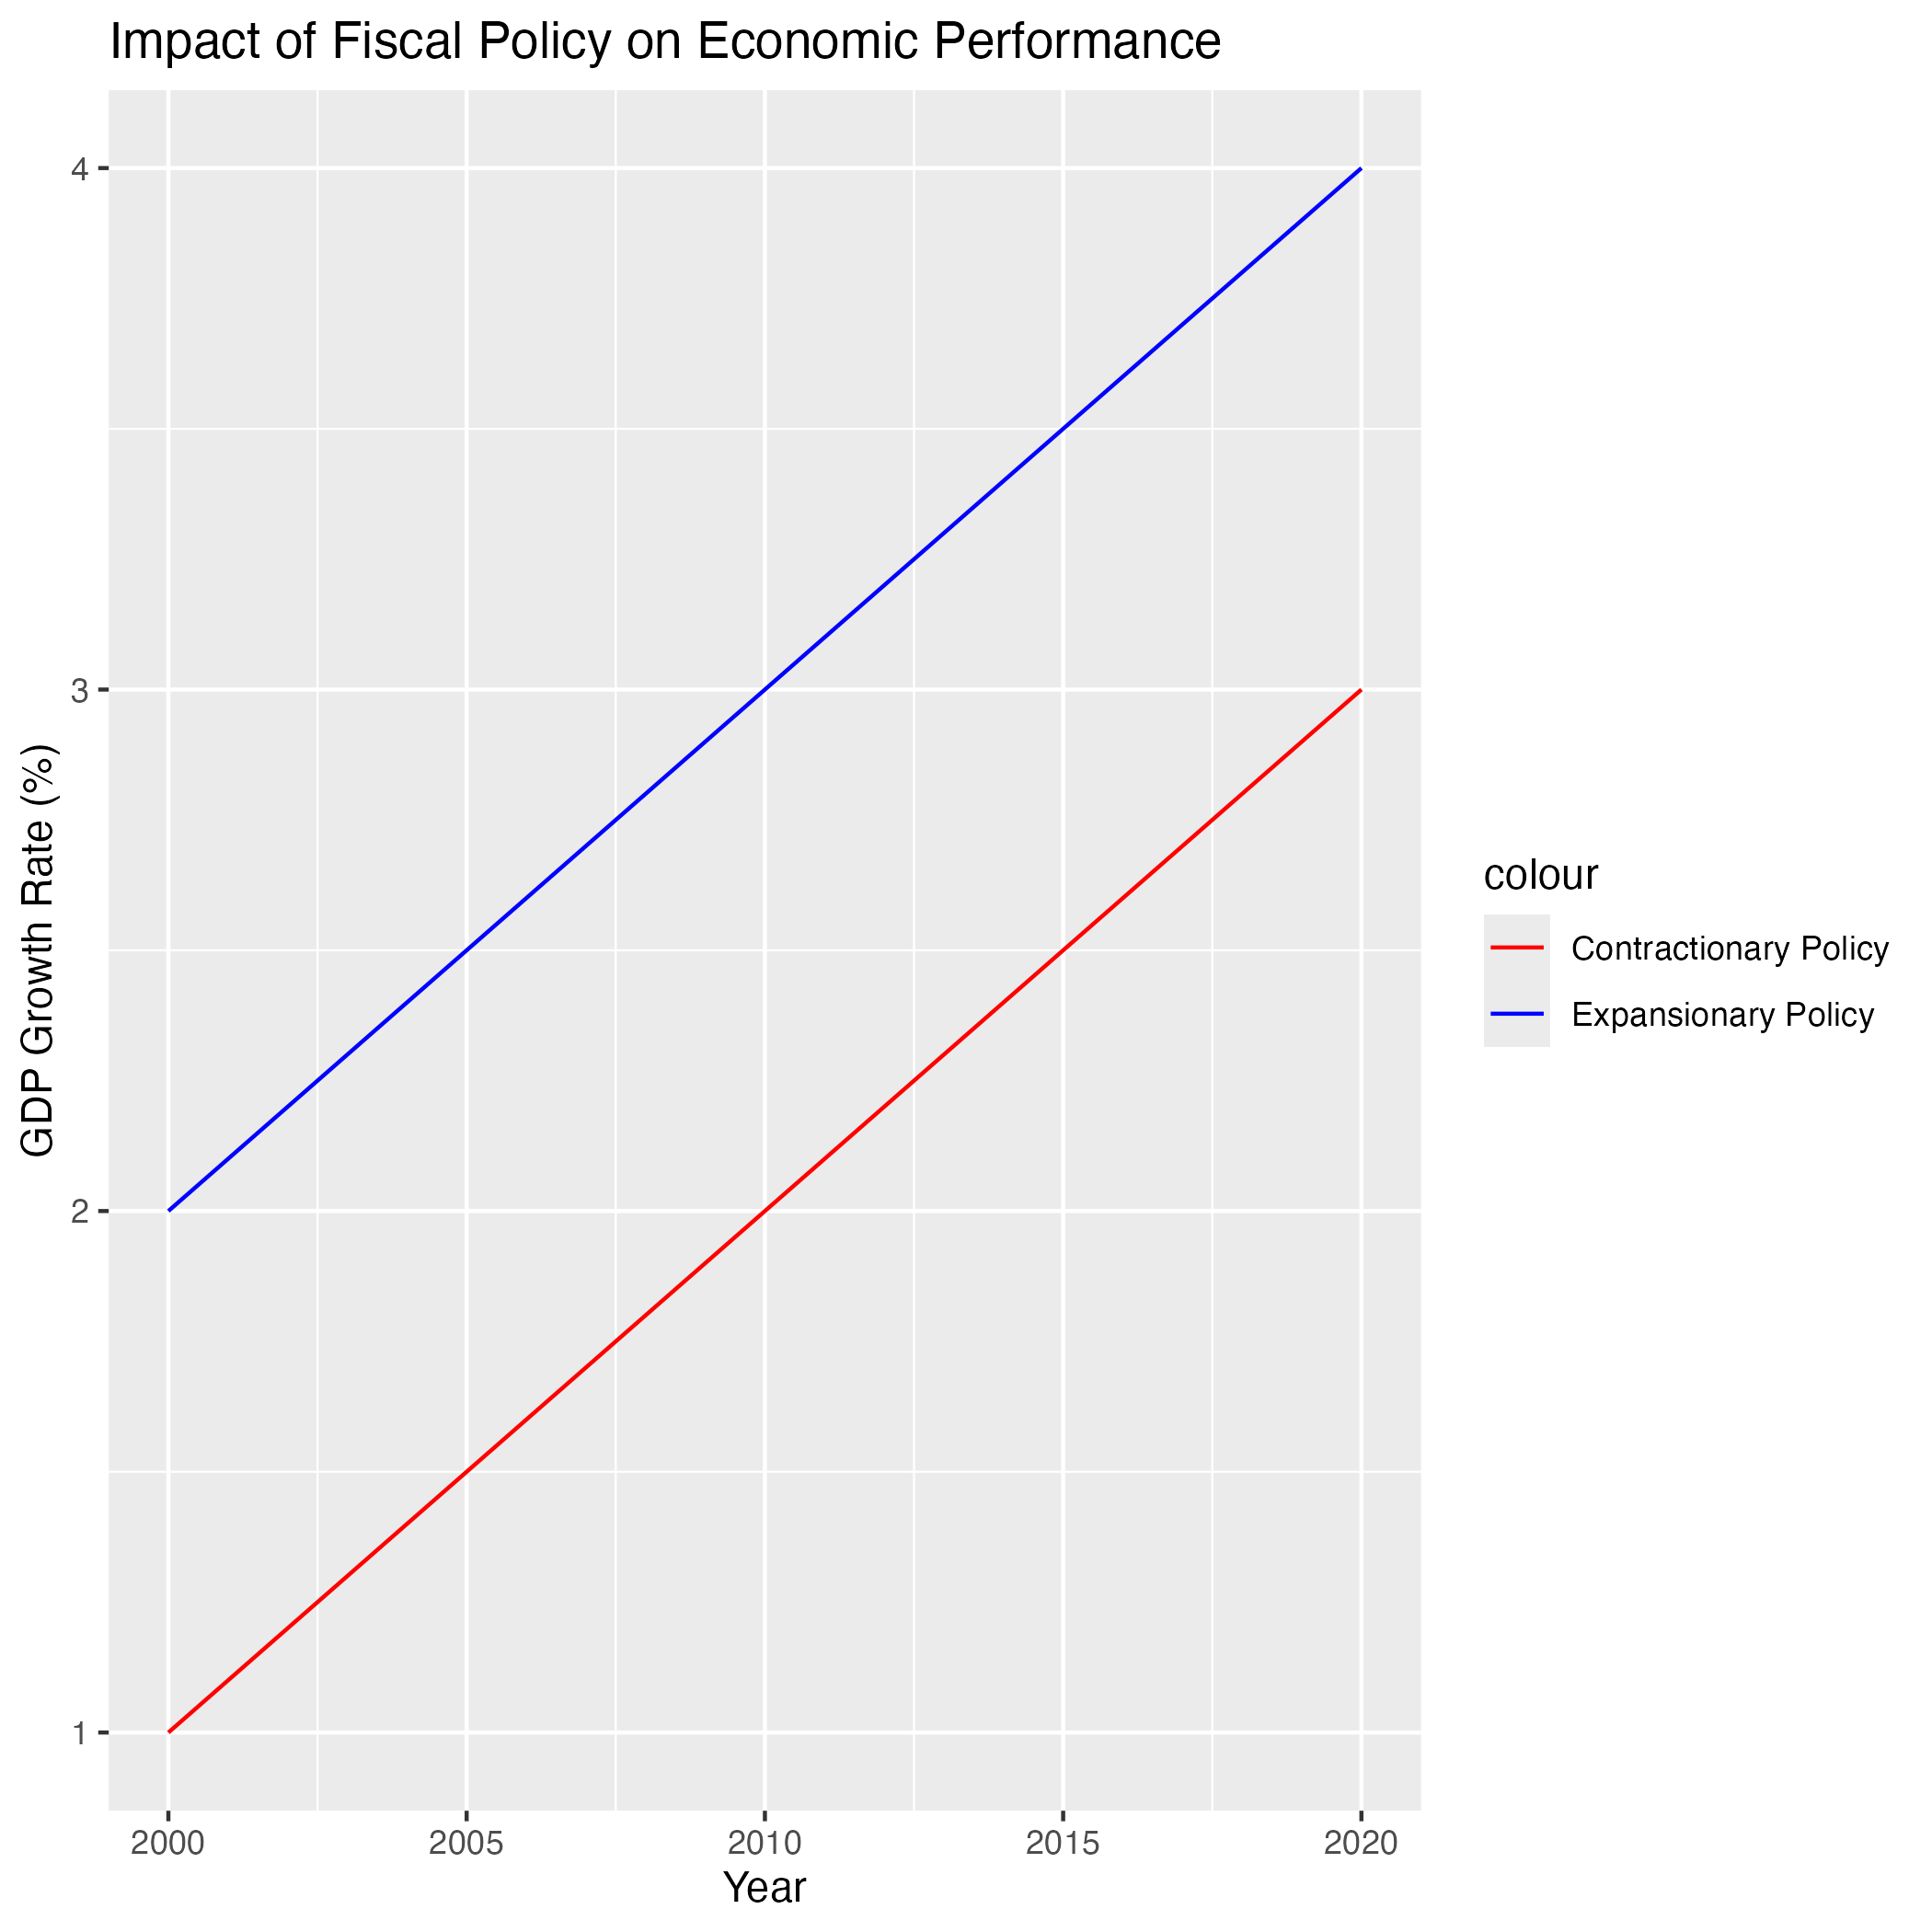
\includegraphics[width=0.8\textwidth]{/Users/cancel/Personal/Coursework/Econ425/VA3/R/Fiscal_Policy_Impact.png}
    \end{figure}
\end{frame}

\begin{frame}
    \frametitle{Key Takeaways: Support for Fiscal Policy}
    \textbf{Key Takeaways:}
    \begin{itemize}
        \item Fiscal policy is essential for economic stabilization.
        \item Public investment can promote long-term growth.
        \item Effective fiscal policy considers both short-term and long-term impacts.
    \end{itemize}
\end{frame}

\section{Conclusion}

\begin{frame}
    \frametitle{Conclusion}
    \begin{itemize}
        \item Thank you for your attention. This concludes my discussion on fiscal policy concepts. If you have any questions, please feel free to ask.
    \end{itemize}
\end{frame}

\end{document}
